
%(BEGIN_QUESTION)
% Copyright 2007, Tony R. Kuphaldt, released under the Creative Commons Attribution License (v 1.0)
% This means you may do almost anything with this work of mine, so long as you give me proper credit

The following functional diagrams represent different controller options in a flow control loop.  Identify each of the features:

$$\includegraphics[width=15.5cm]{i01792x01.eps}$$

\underbar{file i01792}
%(END_QUESTION)





%(BEGIN_ANSWER)

{\bf Left diagram:} Regular PID controller.

\vskip 10pt

{\bf Center diagram:} PID controller with derivative calculated on PV only (not error).

\vskip 10pt

{\bf Right diagram:} PI controller with setpoint tracking.

%(END_ANSWER)





%(BEGIN_NOTES)

The absence of explicit setpoint tracking on the left-hand diagram does not necessarily mean this controller lacks the feature of setpoint tracking.  Like P\&ID's, functional diagrams may omit details for the sake of simplicity.

%INDEX% Documentation, functional: controller symbol identification

%(END_NOTES)


